\chapter{The liquid argon time projection chamber (\lartpc)\label{chap:lartpc}}

The time projection chamber (TPC) is a derivative of Charpak's multi-wire proportional chamber (MWPC)\cite{mwpc} developed by Nygren in 1968~\cite{sauce}.
Passing charged particles ionise the detection medium which was gaseous in the original design.
To prevent the recombination of the ions and electrons, an electric field is applied.
In this field, the electrons drift towards a two-dimensional readout plane.
Originally, the readout was an MWPC.
The charge readout is triggered by a scintillation light readout which also provides accurate timing of an event.
Using this, one can measure the time for the ionisation electrons to reach the readout plane.
Because the drift speed of charged particles in the detection medium is constant, the coordinate in drift direction can be calculated from the drift time if the drift speed is known.

While gaseous TPCs already provide very accurate tracking, they have the disadvantage that the mass and thus the cross-section of the detection medium is quite low resulting in a low interaction rate.
Therefore, Rubbia in 1977 proposed to use liquid argon as a detection medium~\cite{lartpc}.
In turn, this requires a cryogenic detector while gaseous detectors can be operated at room temperature.


\section{Liquid argon (\lar) as a detection medium\label{sec:lartpc_lar}}

For an efficient particle detection by a TPC, its medium needs to fulfil a set of requirements.
As it turns out, \lar\ is quite unique as it has all the necessary properties while at the same time it is comparably cheap.
This section shall outline the most important one of those properties.
A summary can be found in Table~\ref{tab:lartpc_larprop}.

\begin{table}[htb]
	\centering
	\caption{Properties of \lar~\cite{NobleGasDetectors}}
	\label{tab:lartpc_larprop}
	\begin{tabular}{|ll|Ss|}
		\hline
		{Molar mass} &									$\mu$ &					3.9948e1 &	\gram\per\mol \\
		\hline
		{Boiling point at} \SI{1.01325e5}{\pascal} &	$T_{\m{S}}$ &			8.726e1 &	\kelvin \\
		\hline
		{Density at} $T_{\m{S}}$ &						$\rho_{\m{S}}$ &		1.399e3 &	\kilo\gram\per\cubic\metre \\
		\hline
		{Dielectric constant} &							$\varepsilon_{\m{r}}$ &	1.59 &		\\
		\hline
		{Required energy per electron-ion pair} &		$W_{\m{i}}$ &			2.36e1 &	\electronvolt \\
		\hline
		{Fano factor} &									$F$ &					1.07e-1 &	\\
		\hline
		{Radiation length} &							$X_{\m{0}}$ &			1.4e-1 &		\metre \\
		\hline
		{Interaction length} &							$\lambda$ &				8.37e-1 &	\metre \\
		\hline
		{Concentration in air by volume} &				&						9.34e-1 &	\percent \\
		\hline
	\end{tabular}
\end{table}

In order to register the ionisations tracks of charged particles in a TPC, two processes are crucial: production and transportation of charge.
The charge production needs to be high enough to be detectable by the available electronics.
This is given by the energy required to produce an electron-ion pair $W_{\m{i}}$.
As will be shown in Section~\ref{sec:lartpc_electronics}, the value of \SI{23.6}{\electronvolt} for \lar\ is challenging but achievable with contemporary electronics.
Naturally, this imposes a lower limit on detectable $\frac{\m{d}E}{\m{d}x}$.

Charge transport is influenced by multiple factors.
The ultimate goal is to collect as much of the produced charge as possible.
Recombination is the main process opposing this.
While it can be partially mitigated by increasing the electric field, it cannot be eliminated completely.
Even if that was possible, it would not be beneficial because the scintillation light needed for the drift time measurement is partly produced by recombining electron-ion pairs.
The relation between the strength of the drift field and charge yield can be described by the \emph{box model}~\cite{box-model}.
It assumes that the ion-electron pairs are isolated and initially uniformly populate a box of a given size.
Furthermore, the diffusion of electrons and ions as well as the ion drift velocity (\num{1e5} times smaller than for electrons) are assumed to be negligible.
For a produced charge $Q_{\m{0}}$ and a collected charge $Q$, the collection ratio is given by
\begin{IEEEeqnarray}{rCl}
	\frac{Q}{Q_{\m{0}}} & = & \frac{1}{\xi} \ln(1 + \xi)
\end{IEEEeqnarray}
with a parameter $\xi$ depending on the drift field, the electron mobility, the initial number of ion-electron pairs, the chosen size of the box and the recombination coefficient.
Figure~\ref{fig:lartpc_box-model} shows a measurement by LHEP of the collected charge in an \SI{8}{\milli\metre} drift \lartpc\ for different drift field intensities and nitrogen concentrations.

\begin{figure}
	\centering
	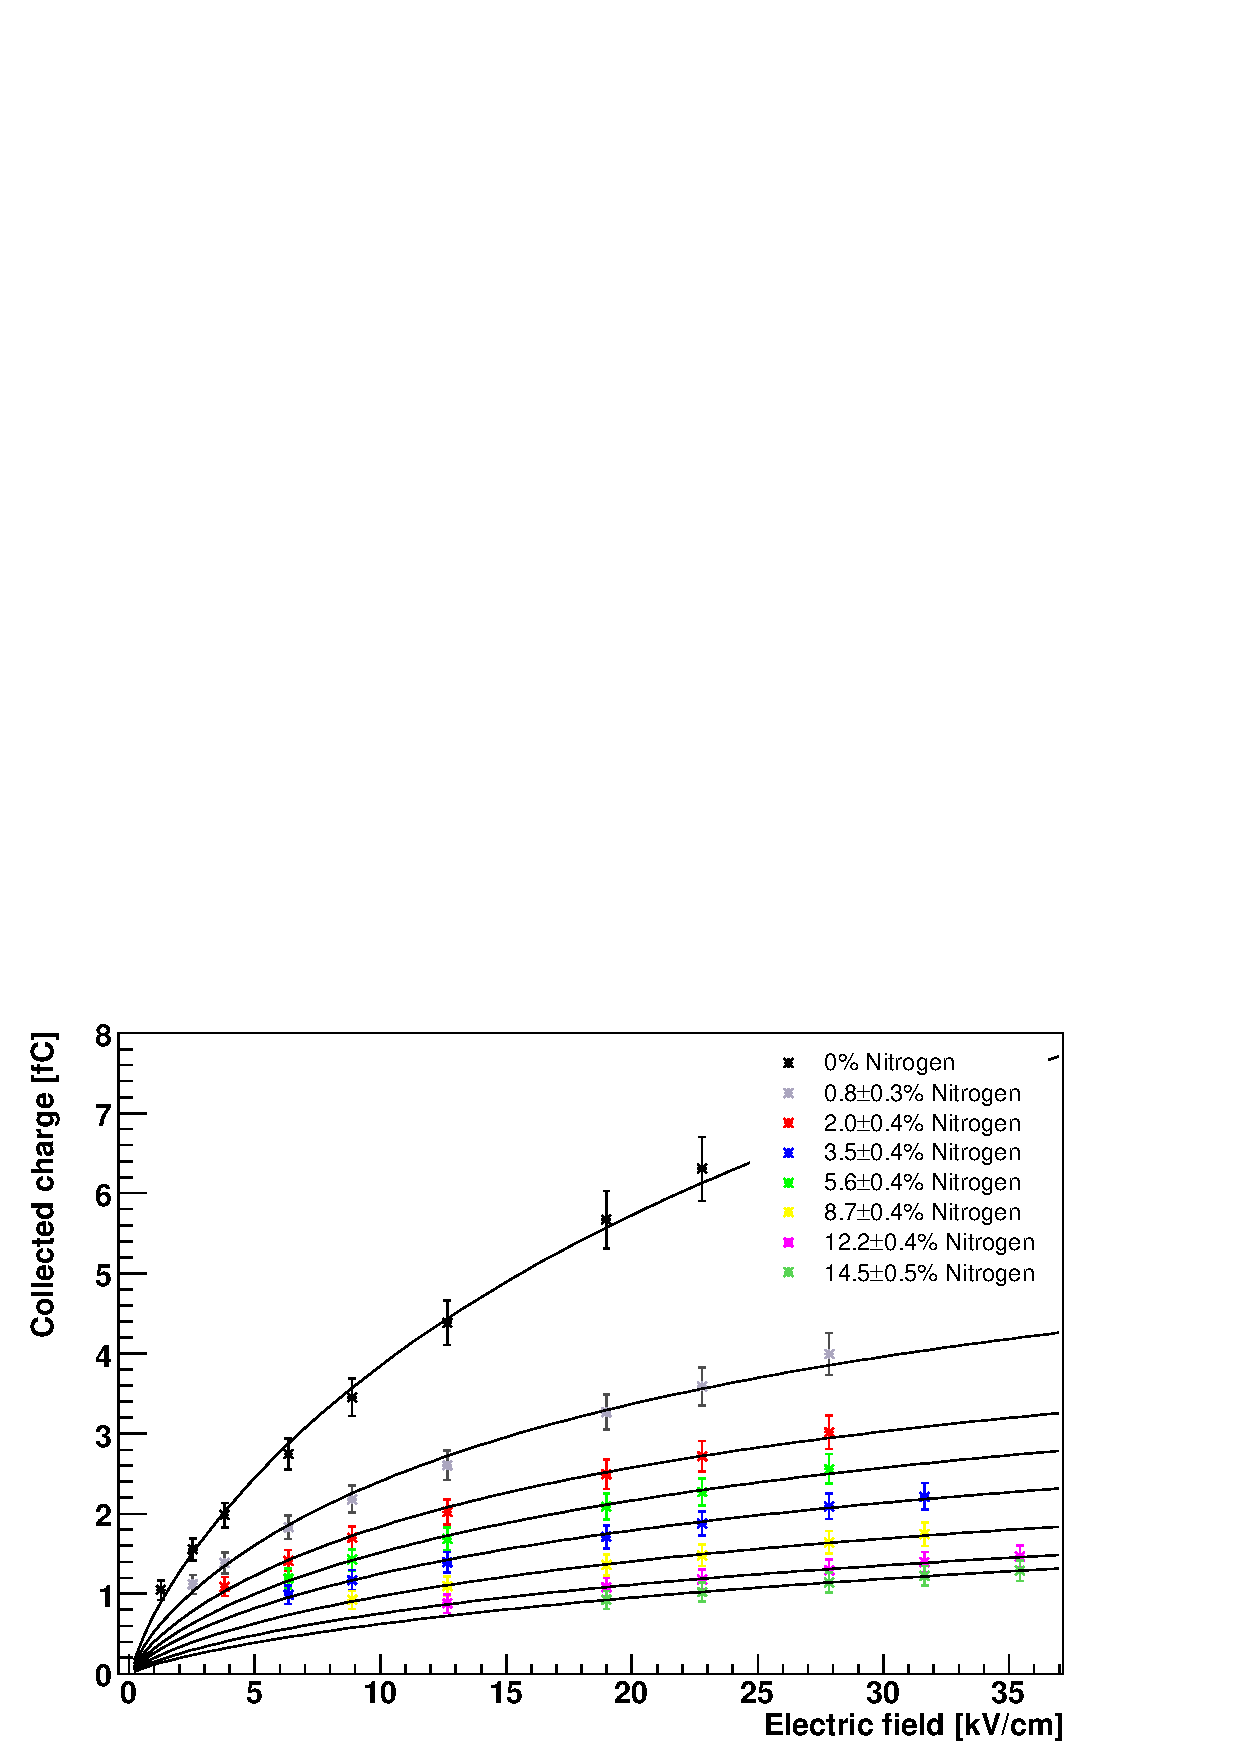
\includegraphics[viewport=14 5 511 351, clip, width=\textwidth]{lartpc/box-model}
	\caption{Collected charge in an \SI{8}{\milli\metre} drift \lartpc\ for different drift field intensities and nitrogen concentrations.
		The lines represent box model fits.~\cite{grna-lhep}}
	\label{fig:lartpc_box-model}
\end{figure}

A second process affecting charge transport is electron trapping by impurities.
The probability of an electron becoming attached to an atom in the medium.
For the argon itself, this is highly unlikely because its outer electron shell is fully populated.
This is one or the reasons why (liquefied) noble gases are a prime choice for TPCs.
Nevertheless, drifting electron can be captured by impurities in the argon.
A particularly bad one oxygen due to its high electronegativity.
Therefore, it is very important to keep the detection medium very pure.

The velocity of the charge drifting in an electric field is related to the so-called mobility by

\begin{IEEEeqnarray}{rCl}
	\va{v} & = & \mu\qty(\va{E}) \va{E}
\end{IEEEeqnarray}

where the mobility $\mu$ in general depends on the electric field.
This means, the higher the field is, the higher the charge velocity and thus, the drift time.
One wants to keep drift times low for multiple reasons.
One of them are the aforementioned impurities.
They cause the charge to posses a finite lifetime following an exponential decay with time.
The consequence is that higher impurities can be partially compensated by a higher field.
In a beam experiment with a given beam timing, increasing the drift time will increase pile-up, i.e. the number of events simultaneously present in the detector.
Pile-up in turn, makes event reconstruction more complicated.
On the other hand, the readout electronics need to be fast enough to guarantee the required spatial resolution in the drift coordinate which defines an upper limit for the drift velocity.
A reasonable value from a purity point of view is a drift time of $\order{\SI{1}{\milli\second}}$.
For a detector size of $\order{\SI{1}{\metre}}$, the required drift speed is $\order{\SI{1}{\milli\metre\per\micro\second}}$ which requires a field of $\order{\SI{1}{\kilo\volt\per\centi\metre}}$.

For detectors much larger than \SI{1}{\metre}, a drift field of \SI{1}{\kilo\volt\per\centi\metre} becomes challenging due to the required high cathode voltage.
Soon after entering \lartpc\ R\&D, the Bern group realised that the reported dielectric strength of \lar\ is much lower~\cite{breakdown_14} than measured by Swan et al.\ in 1960~\cite{swan1, swan2}.
It turned out, opposing the assumption of Swan et al., that the dielectric strength is not independent of the absolute dimensions of the electrodes.
This led to a very detailed study of breakdowns in \lar\ in the course of this thesis which is presented in Chapter~\ref{chap:hv}.


\begin{itemize}
	\item General specs
	\item Electronegativity
	\item Ionisation
	\item Scintillation
	\item Recombination
	\item Diffusion
	\item Dielectric strength
\end{itemize}
\cite{NobleGasDetectors}


\section{Electric field generation\label{sec:lartpc_efield}}

For charge separation and drift, an electric field of $\order{\SI{1}{\kilo\volt\per\centi\metre}}$ is needed inside the fiducial volume of a \lartpc.
An easy way to achieve this is by means of field shaping rings fed by a resistive divider between cathode and anode.
The drawback is the need for a feedthrough capable of withstanding the full cathode voltage.
One alternative is to generate the high voltage inside the cryostat, for instance using a Greinacher voltage multiplier circuit as the one used for the \AT\ experiment at LHEP at the University of Bern~\cite{AT}.
A Greinacher multiplier works by pumping up a cascade of capacitors and diodes using a high frequency source.
However, while the voltage generation itself worked well, this approach proofed to be impractical because the high frequency voltage needed to charge the multiplier interfered with the readout and therefore had to be turned off during data-taking.
Recharging, in turn, caused a lot of detector down time.


\section{Charge readout\label{sec:lartpc_charge-ro}}

Classically, the charge readout of a liquid argon TPC is done using wires with a diameter of the order of \SI{100}{\micro\metre}.
One wire plane delivers a 2D projection of the ionisation tracks in the detection medium.
This has two consequences:
\begin{enumerate}
	\item At least two parallel wire planes are needed to be able to reconstruct the 3D event topology.
	\item In theory, the higher the complexity of the event, the more planes would be required to be able to fully reconstruct it.
\end{enumerate}
Multiple wire planes can be realised by operating only the last one (in drift direction) in charge collection mode.
All the preceeding wire planes are biased in a such a way that they are transparent to the incoming charge but pick up an induction signal during the passage of the latter.
A typical number of wire planes for currently operational detectors is three.
They are tilted by \SI{60}{\degree} against each other.


\section{Light readout\label{sec:lartpc_light-ro}}

In order to calculate the distance, the charge has drifted along the electric field (i.e.\ the space coordinate perpendicular to the readout plane), one needs to record the drift time.
The data acquisition can record the time of the arrival of the charge at the readout plane.
What is missing is the time of the charge production.
This can be acquired by registering the scintillation light produced alongside the ionisation of the detection medium.
Contemporary detector designs employ photomultiplier tubes (PMTs) for this purpose.
PMTs are a well established technology with a high quantum efficiency and a fast response.

The light impinging upon a PMT is converted to an electron by a photo cathode coated on the sensitive window of the PMT.
These photo cathodes have a limited absorption spectrum.
In particular, the scintillation light of \lar\ does not fall inside this spectrum for most photo cathodes.
That is why the vacuum UV scintillation light needs to be converted to the visible range where it can be efficiently detected by a PMT.
A widespread wavelength-shifter capable of achieving this is tetraphenyl butadiene (TPB).
Therefore, a common setup consists of a surface of TPB in front of a PMT.


\section{Electronics\label{sec:lartpc_electronics}}

Using the energy required to produce one electron ion pair $W_{\m{i}}$ from Section~\ref{sec:lartpc_lar} and assuming a MIP, one gets

\begin{IEEEeqnarray*}{rCl}
	\dv{Q}{x}	= \frac{\eval{\dv{E}{x}}_{\m{MIP}}}{W_{\m{i}}} \si{\elementarycharge}
									&	= & \frac{\SI{2}{\mega\electronvolt\per\centi\metre}}{\SI{23.6}{\electronvolt}} \si{\elementarycharge}
											\approx \SI{8500}{\elementarycharge\per\milli\metre}
											\approx \SI{1.4}{\femto\coulomb\per\milli\metre}
\end{IEEEeqnarray*}

as a rough estimation for the charge yield.
This calculation does not incorporate recombination, meaning that in a real experiment the value will be even lower.
The result is that the readout electronics need to be capable of detecting charge in the order of \si{\femto\coulomb}.

That is why the charge signal needs to be amplified before digitisation.
This is achieved by means of an integrating amplifier which also converts the charge to a voltage.
Early \lartpc\ designs used preamplifiers outside the cryostat at room temperature for this.
From a noise point of view though, it is beneficial to put the amplifiers inside the cryostat emerged in \lar\ for two reasons.
First off, the closer to the source the amplifier is located, the shorter the low-signal lines will be, resulting in less pick-up noise.
An additional advantage is that the temperature-dependent Johnson-Nyquist noise of the amplifiers will be reduced at cryogenic temperatures.

For the same reasons it might even make sense to operate the entire analogue signal chain at cryogenic temperatures.
This would also help to eliminate ground loops which can pick-up noise inductively or provoke self-oscillation of the analog signal circuitry.
On the other hand, in general it is not easy to operate a circuit at cryogenic temperatures.
Usually, a complete redesign of the circuit is necessary due to most components operating outside their guaranteed temperature range.
For some complex active components like the amplifiers and ADCs, even a redesign of the integrated circuit might be necessary.
On the other hand, placing the digitisers too close to the readout might result in elevated noise levels due to the digital clocks coupling into the analogue signal path.

The requirements on the electronics are given by the required sensitivity of the detector.
The necessary bit depth of the ADCs is given by the required dynamic range, i.e.\ the minimum and maximum amount of charge the readout needs to be able to register.
While the spatial resolution in the two coordinates parallel to the readout plane is given by the pitch of the electrodes, the accuracy of the third coordinate is given by the timing accuracy.
This in turn depends on three properties: the timing accuracy of the light readout, the sampling time of the ADCs and the peaking time of the preamplifiers.
Peaking time is the time needed until the output of the preamplifier reaches its maximum (peak) for a delta pulse input.


\section{Challenges of future detectors\label{sec:lartpc_challenges}}
To accomplish the physics goals of future neutrino detectors, outlined in Chapter~\ref{chap:introduction}, much higher statistics than with today's experiments are necessary.
There are two obvious ways to do this: Increase the flux and the detector size.